\documentclass{beamer}

\usetheme{boxes}
\definecolor{beamer@structure@color}{rgb}{0,0,0}

\usecolortheme{structure}

\setbeamertemplate{footline}[frame number]
\setbeamertemplate{frametitle}{\color{black}
\def\myhrulefill{\leavevmode\leaders\hrule height 1pt\hfill\kern 0pt}
\headingfont\insertframetitle\par\vskip-8pt\myhrulefill}

\newcommand{\ZZ}{\mathbb{Z}}
\newcommand{\QQ}{\mathbb{Q}}
\renewcommand{\O}{\mathcal{O}}

\setbeamertemplate{navigation symbols}{}

\usepackage{mathspec}
\setmainfont{Montserrat}
\setsansfont{Montserrat}
\setmonofont{PT Mono}
\newfontfamily\headingfont[]{Montserrat Bold}

\usepackage{xcolor}
\usepackage{framed}
\definecolor{shadecolor}{rgb}{0.945, 0.902, 0.698}

\begin{document}

%%%%%%%%%%%%%%%%%%%%%%%%%%%%%%%%%%%%%%%%%%%%%%%%%%%%%%%%%%%%%%%%%%%%%%%%%%%%%%%%

\begin{frame}[noframenumbering]
  \headingfont
  \begin{center}
    {\huge Teoría de números

      algebraicos

      en PARI/GP

    }

    \vspace{3em}

    {\large Parte I: campos de números, anillos de enteros}

    \vspace{3em}

    23/09/2020

  \end{center}
\end{frame}

%%%%%%%%%%%%%%%%%%%%%%%%%%%%%%%%%%%%%%%%%%%%%%%%%%%%%%%%%%%%%%%%%%%%%%%%%%%%%%%%

\begin{frame}
  \frametitle{PARI/GP}

  \begin{itemize}
  \item Sistema de álgebra computacional

  \item Enfoque en la teoría de números

  \item \url{https://pari.math.u-bordeaux.fr/}
  \end{itemize}

  \begin{center}
    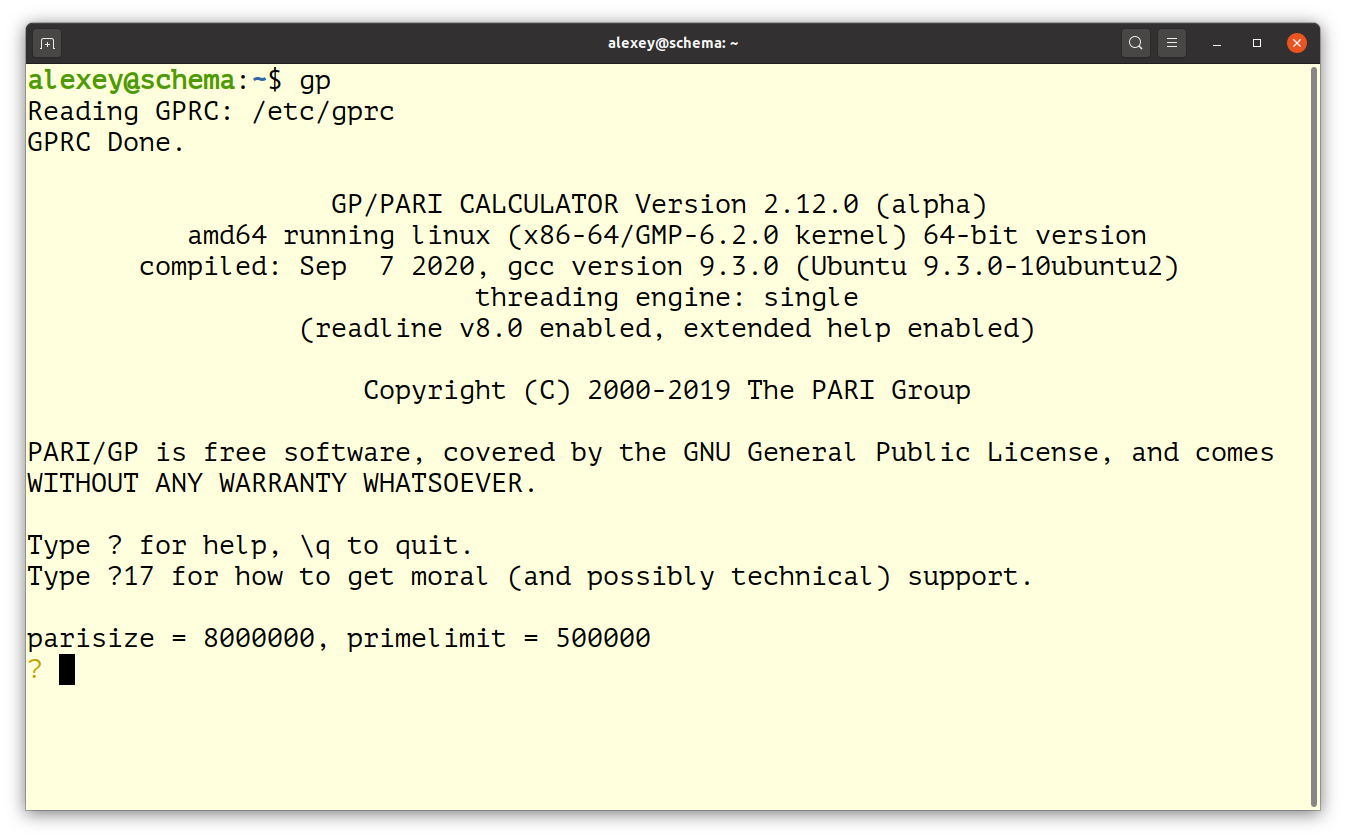
\includegraphics[width=9cm]{pari-terminal.png}
  \end{center}
\end{frame}

%%%%%%%%%%%%%%%%%%%%%%%%%%%%%%%%%%%%%%%%%%%%%%%%%%%%%%%%%%%%%%%%%%%%%%%%%%%%%%%%

\begin{frame}
  \frametitle{¿Cómo funciona?}

  \begin{center}\setlength{\fboxsep}{0pt}\setlength{\fboxrule}{0.5pt}
    \fbox{
\includegraphics[width=5cm]{gtm-138.jpg}}
  \end{center}

\end{frame}

%%%%%%%%%%%%%%%%%%%%%%%%%%%%%%%%%%%%%%%%%%%%%%%%%%%%%%%%%%%%%%%%%%%%%%%%%%%%%%%%

\begin{frame}[fragile]
  \frametitle{Comandos útiles}

  \begin{itemize}
  \item $\boxed{\rightarrow}$ --- completar la palabra

  \item \texttt{\textbackslash{}l "log.txt"} --- guardar la sesión en
    \texttt{log.txt}

  \item Otra vez \texttt{\textbackslash{}l} --- dejar de hacerlo

  \item \texttt{?xxxxx} --- ayuda sobre \texttt{xxxxx}

    \texttt{??xxxxx} --- ayuda detallada

  \item \texttt{\textbackslash{}quit} --- salir del programa
  \end{itemize}

  \begin{shaded}\small
\begin{verbatim}
? ?idealprimedec
idealprimedec(nf,p,{f=0}): prime ideal 
decomposition of the prime number p in the 
number field nf as a vector of prime ideals. 
If f is present and non-zero, restrict the 
result to primes of residue degree <= f.
\end{verbatim}
\end{shaded}
\end{frame}

%%%%%%%%%%%%%%%%%%%%%%%%%%%%%%%%%%%%%%%%%%%%%%%%%%%%%%%%%%%%%%%%%%%%%%%%%%%%%%%%

\begin{frame}[fragile]
  \frametitle{Resultado de cálculo}

  \begin{itemize}
  \item \texttt{\%} --- resultado del cálculo anterior
  \end{itemize}

  \begin{shaded}
\begin{verbatim}
? 2^2
%1 = 4
? %^2
%2 = 16
? %^2
%3 = 256
? %1 + %2
%4 = 20
\end{verbatim}
  \end{shaded}
\end{frame}

%%%%%%%%%%%%%%%%%%%%%%%%%%%%%%%%%%%%%%%%%%%%%%%%%%%%%%%%%%%%%%%%%%%%%%%%%%%%%%%%

\begin{frame}[fragile]
  \frametitle{Cuando algo va mal\dots}

  \begin{shaded}
\begin{verbatim}
? mcd(2,3)
  ***   at top-level: mcd(2,3)
  ***                 ^--------
  ***   not a function in function call
  ***   Break loop: type 'break' to go back
  ***   to GP prompt
break> break

? gcd(2,3)
% = 1
\end{verbatim}
  \end{shaded}
\end{frame}

%%%%%%%%%%%%%%%%%%%%%%%%%%%%%%%%%%%%%%%%%%%%%%%%%%%%%%%%%%%%%%%%%%%%%%%%%%%%%%%%

\begin{frame}[plain]
  \headingfont

  \begin{center}
    {\huge Polinomios}
  \end{center}
\end{frame}

%%%%%%%%%%%%%%%%%%%%%%%%%%%%%%%%%%%%%%%%%%%%%%%%%%%%%%%%%%%%%%%%%%%%%%%%%%%%%%%%

\begin{frame}[fragile]
  \frametitle{Irreducibilidad}

  \begin{shaded}
\begin{verbatim}
? polisirreducible(x^3 - 3*x + 1)
% = 1
? polisirreducible(x^4 + x^3 + x^2 + x + 1)
% = 1
? polisirreducible(x^3 + x^2 + x + 1)
% = 0
\end{verbatim}
  \end{shaded}
\end{frame}

%%%%%%%%%%%%%%%%%%%%%%%%%%%%%%%%%%%%%%%%%%%%%%%%%%%%%%%%%%%%%%%%%%%%%%%%%%%%%%%%

\begin{frame}[fragile]
  \frametitle{Factorización}

  \begin{shaded}\small
\begin{verbatim}
? factor (x^8-1)
% = 
[  x - 1 1]
[  x + 1 1]
[x^2 + 1 1]
[x^4 + 1 1]

? factor (x^3 + x^2 - x - 1)
% = 
[x - 1 1]
[x + 1 2]
\end{verbatim}
  \end{shaded}
\end{frame}

%%%%%%%%%%%%%%%%%%%%%%%%%%%%%%%%%%%%%%%%%%%%%%%%%%%%%%%%%%%%%%%%%%%%%%%%%%%%%%%%

\begin{frame}[fragile]
  \frametitle{Polinomios mód p}

  \begin{itemize}
    \item \texttt{$f$*Mod(1,$p$)} --- reducción mód $p$ para $f \in \ZZ_{(p)} [x]$
  \end{itemize}

  \begin{shaded}\small
\begin{verbatim}
? factor (polcyclo(8)*Mod(1,2))
% = 
[Mod(1, 2)*x + Mod(1, 2) 4]

? factor (polcyclo(8)*Mod(1,3))
% = 
[Mod(1, 3)*x^2 + Mod(1, 3)*x + Mod(2, 3) 1]
[Mod(1, 3)*x^2 + Mod(2, 3)*x + Mod(2, 3) 1]

? factor (polcyclo(8)*Mod(1,5))
% = 
[Mod(1, 5)*x^2 + Mod(2, 5) 1]
[Mod(1, 5)*x^2 + Mod(3, 5) 1]
\end{verbatim}
  \end{shaded}
\end{frame}

%%%%%%%%%%%%%%%%%%%%%%%%%%%%%%%%%%%%%%%%%%%%%%%%%%%%%%%%%%%%%%%%%%%%%%%%%%%%%%%%

\begin{frame}[fragile]
  \frametitle{Discriminante}

  \begin{itemize}
  \item $\Delta (f)$ = \texttt{poldisc($f$)}
  \end{itemize}

  \begin{shaded}
\begin{verbatim}
? poldisc (polcyclo(7))
% = -16807
? factor(%)
% = 
[-1 1]

[ 7 5]
\end{verbatim}
  \end{shaded}
\end{frame}

%%%%%%%%%%%%%%%%%%%%%%%%%%%%%%%%%%%%%%%%%%%%%%%%%%%%%%%%%%%%%%%%%%%%%%%%%%%%%%%%

\begin{frame}[plain]
  \headingfont

  \begin{center}
    {\huge Campos de números}
  \end{center}
\end{frame}

%%%%%%%%%%%%%%%%%%%%%%%%%%%%%%%%%%%%%%%%%%%%%%%%%%%%%%%%%%%%%%%%%%%%%%%%%%%%%%%%

\begin{frame}[fragile]
  \frametitle{nfinit}

  $f \in \QQ [x]$ irreducible.

  Especificar $K = \QQ[x]/(f)$, calcular invariantes básicos:

  \begin{center}
    \texttt{$K$=nfinit($f$);}
  \end{center}

  \vspace{\fill}

  * \texttt{nf} = \emph{number field}.

  \vspace{\fill}

  Algunos invariantes:
  \begin{itemize}
  \item \texttt{$K$.pol} --- polinomio $f$

  \item \texttt{$K$.zk} --- $\ZZ$-base $\O_K$ en términos de la $\QQ$-base
    $1,x,x^2,\ldots,x^{n-1} \pmod{f}$

  \item \texttt{$K$.disc} --- discriminante $\Delta_K$

  \item \texttt{$K$.sign} --- signatura \texttt{[$r_1$,$r_2$]}
  \end{itemize}
\end{frame}

%%%%%%%%%%%%%%%%%%%%%%%%%%%%%%%%%%%%%%%%%%%%%%%%%%%%%%%%%%%%%%%%%%%%%%%%%%%%%%%%

\begin{frame}[fragile]
  \frametitle{Ejemplo: $\QQ (\sqrt[3]{19})$}

  \begin{shaded}\footnotesize
\begin{verbatim}
? K = nfinit(x^3-19);
? K.sign
% = [1, 1]
? K.disc 
% = -1083
? factor (%)
% = 
[-1 1]
[ 3 1]
[19 2]

? K.zk
% = [1, 1/3*x^2 + 1/3*x + 1/3, x]
\end{verbatim}
  \end{shaded}

  $$\O_K = \ZZ \oplus \frac{1}{3} (\alpha^2 + \alpha + 1) \ZZ \oplus \alpha \ZZ.$$
\end{frame}

%%%%%%%%%%%%%%%%%%%%%%%%%%%%%%%%%%%%%%%%%%%%%%%%%%%%%%%%%%%%%%%%%%%%%%%%%%%%%%%%

\begin{frame}[fragile]
  \frametitle{Para qué sirve punto y coma}

  \begin{center}
    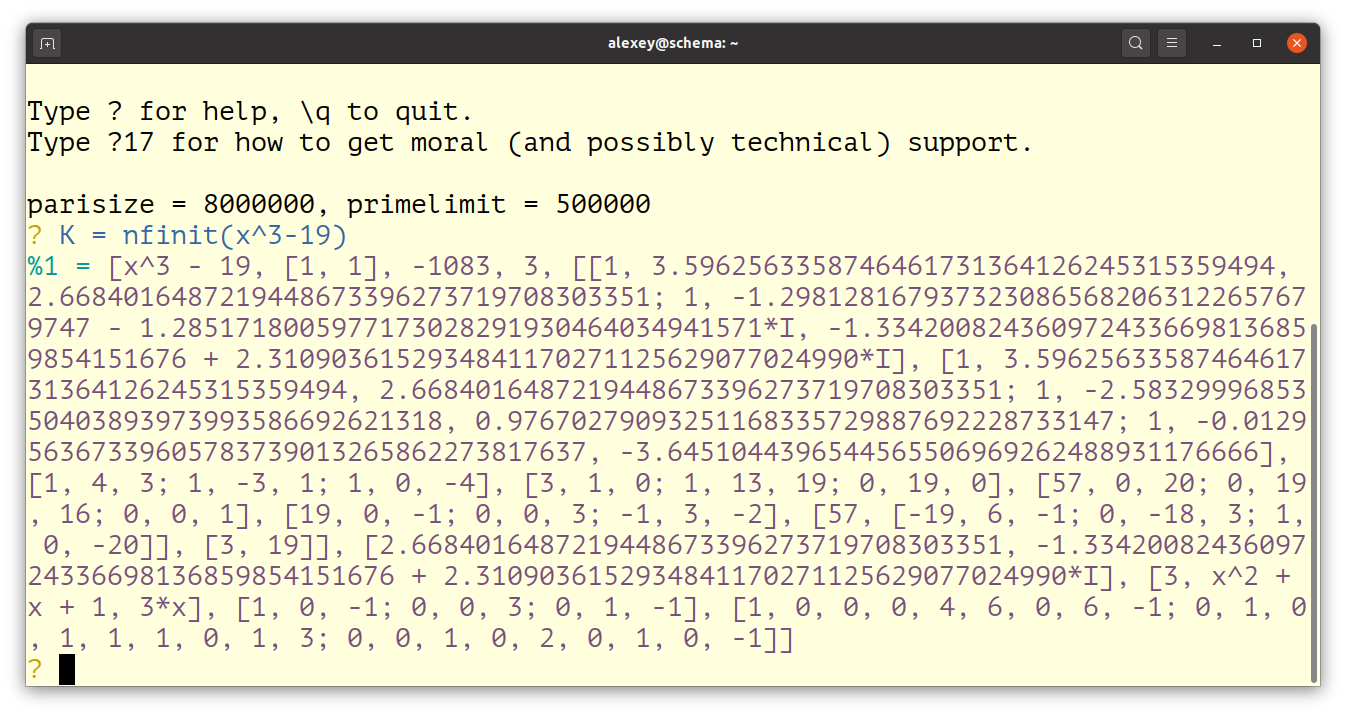
\includegraphics[width=11cm]{long-output.png}
  \end{center}
\end{frame}


%%%%%%%%%%%%%%%%%%%%%%%%%%%%%%%%%%%%%%%%%%%%%%%%%%%%%%%%%%%%%%%%%%%%%%%%%%%%%%%%

\begin{frame}[fragile]
  \frametitle{Isomorfismo}

  \begin{itemize}
  \item \texttt{nfisisom($K$,$L$)} --- $K \stackrel{?}{\cong} L$
  \item $K$ y $L$: polinomios irreducibles o estructuras \texttt{nfinit}
  \end{itemize}

  \begin{shaded}\footnotesize
\begin{verbatim}
? nfisisom(x^4 + 2*x^2 + 4*x + 2, polcyclo(8))
% = [x^2 - x, x^2 + x, -x^3 - x^2, x^3 - x^2]

? nfisisom(x^4 + 2, polcyclo(8))
% = 0
\end{verbatim}
  \end{shaded}

  Uno de los isomorfismos:
  \begin{align*}
  \QQ [\alpha]/(\alpha^4 + 2 \alpha^2 + 4 \alpha + 2) & \cong \QQ (\zeta_8),\\
  \alpha & \mapsto \zeta_8^2 - \zeta_8.
  \end{align*}
\end{frame}

%%%%%%%%%%%%%%%%%%%%%%%%%%%%%%%%%%%%%%%%%%%%%%%%%%%%%%%%%%%%%%%%%%%%%%%%%%%%%%%%

\begin{frame}[fragile]
  \frametitle{Inclusión}
  \begin{itemize}
  \item \texttt{nfisincl($K$,$L$)} --- $K \stackrel{?}{\subseteq} L$
  \item $K$ y $L$: polinomios irreducibles o estructuras \texttt{nfinit}
  \end{itemize}

  \begin{shaded}\footnotesize
\begin{verbatim}
? nfisincl(x^2-7, polcyclo(7))
% = 0
? nfisincl(x^2+7, polcyclo(7))
% = [-2*x^4 - 2*x^2 - 2*x - 1, 2*x^4 + 2*x^2 + 2*x + 1]
\end{verbatim}
  \end{shaded}

  Significado: $\QQ (\sqrt{7}) \not\subset \QQ (\zeta_7)$,
  $\QQ (\sqrt{-7}) \subset \QQ (\zeta_7)$.

  \vspace{\fill}

  * Más adelante: teoría de Galois
\end{frame}

%%%%%%%%%%%%%%%%%%%%%%%%%%%%%%%%%%%%%%%%%%%%%%%%%%%%%%%%%%%%%%%%%%%%%%%%%%%%%%%%

\begin{frame}[fragile]
  \frametitle{polredbest}

  \begin{itemize}
  \item \texttt{polredbest($f$)}: polinomio $g$ tal que
    $\QQ[x]/(f) \cong \QQ[x]/(g)$

  \item Coeficientes de $g$ <<pequeños>>
  \end{itemize}
\end{frame}

%%%%%%%%%%%%%%%%%%%%%%%%%%%%%%%%%%%%%%%%%%%%%%%%%%%%%%%%%%%%%%%%%%%%%%%%%%%%%%%%

\begin{frame}[fragile]
  \frametitle{Ejemplo: $K = \QQ (\sqrt{2},\sqrt{3})$}

  \begin{itemize}
  \item $K = \QQ (\alpha)$, $\alpha = \sqrt{2} + \sqrt{3}$

  \item $f^\alpha_\QQ = x^4 - 10 x^2 + 1$
  \end{itemize}

  \begin{shaded}\footnotesize
\begin{verbatim}
? f = x^4 - 10*x^2 + 1;
? poldisc(f)
% = 147456

? K = nfinit(f);
? K.disc 
% = 2304

? sqrtint(poldisc(f)/K.disc)
% = 8
\end{verbatim}
  \end{shaded}

  \[ \ZZ [\alpha] = 2^{14}\cdot 3^2, \quad
     \Delta_K = 2^8\cdot 3^2, \quad
     [\O_K : \ZZ [\alpha]] = 8. \]
\end{frame}

%%%%%%%%%%%%%%%%%%%%%%%%%%%%%%%%%%%%%%%%%%%%%%%%%%%%%%%%%%%%%%%%%%%%%%%%%%%%%%%%

\begin{frame}[fragile]
  \frametitle{¡polredbest!}

  \begin{shaded}\small
\begin{verbatim}
? g = polredbest(f)
% = x^4 - 4*x^2 + 1
? poldisc(g)
% = 2304
? % == K.disc 
% = 1
\end{verbatim}
  \end{shaded}

  \begin{itemize}
    \item Encontramos $\ZZ [\beta]$, $\beta^4 - 4\beta^2 + 1 = 0$
    \item Resulta que $\O_K = \ZZ [\beta]$
  \end{itemize}
\end{frame}

%%%%%%%%%%%%%%%%%%%%%%%%%%%%%%%%%%%%%%%%%%%%%%%%%%%%%%%%%%%%%%%%%%%%%%%%%%%%%%%%

\begin{frame}[fragile]
  \frametitle{Otro ejemplo: $K = \QQ (\sqrt[3]{19})$}
  \begin{shaded}\small
\begin{verbatim}
? f = x^3-19;
? K = nfinit(f);
? sqrtint(poldisc(f)/K.disc)
% = 3
? polredbest(f,1)   /* expr. raíz de f mód g */
% = [x^3 - x^2 - 6*x - 12,
     Mod(1/2*x^2 - 1/2*x - 2, x^3 - x^2 - 6*x - 12)]
? sqrtint(poldisc(%[1])/K.disc)
% = 2
\end{verbatim}
  \end{shaded}

  \begin{itemize}
  \item $[\O_K : \ZZ [\alpha]] = 3$
  \item $\ZZ [\beta] \subset \O_K$, $\beta^3 - \beta^2 - 6\beta - 12 = 0$
  \item $[\O_K : \ZZ [\beta]] = 2$
  \item $\alpha = \frac{1}{2}\beta^2 - \frac{1}{2}\beta - 2$
  \end{itemize}
\end{frame}

%%%%%%%%%%%%%%%%%%%%%%%%%%%%%%%%%%%%%%%%%%%%%%%%%%%%%%%%%%%%%%%%%%%%%%%%%%%%%%%%

\begin{frame}[plain]
  \headingfont

  \begin{center}
    {\huge Elementos de $K/\QQ$}
  \end{center}
\end{frame}

%%%%%%%%%%%%%%%%%%%%%%%%%%%%%%%%%%%%%%%%%%%%%%%%%%%%%%%%%%%%%%%%%%%%%%%%%%%%%%%%

\begin{frame}[fragile]
  \frametitle{En la $\QQ$-base $1,x,x^2,\ldots,x^{n-1}$}

  Elemento $\alpha \in \QQ[x]/(f)$ $\longleftrightarrow$ polinomio $g \in \QQ [x]$ módulo $f$

  \begin{shaded}\small
\begin{verbatim}
? a = Mod(x^4 - x^3 - x^2 + x, polcyclo(5))
% = Mod(-2*x^3 - 2*x^2 - 1, x^4 + x^3 + x^2 + x + 1)
? a^2
% = Mod(5, x^4 + x^3 + x^2 + x + 1)
\end{verbatim}
  \end{shaded}
\end{frame}

%%%%%%%%%%%%%%%%%%%%%%%%%%%%%%%%%%%%%%%%%%%%%%%%%%%%%%%%%%%%%%%%%%%%%%%%%%%%%%%%

\begin{frame}[fragile]
  \frametitle{En la $\ZZ$-base de $\O_K$}

  \begin{itemize}
  \item \texttt{$K$.zk}: $\ZZ$-base de $\O_K$ calculada por \texttt{nfinit}

  \item $\O_K = \alpha_1 \ZZ \oplus \cdots \oplus \alpha_n \ZZ$

  \item $\alpha \in K$ $\longleftrightarrow$ $\QQ$-vector
    \texttt{[$a_1$, \ldots, $a_n$]\textasciitilde}

  \item $\alpha = a_1 \alpha_1 + \cdots + a_n \alpha_n$

  \item \texttt{[$a_1$, \ldots, $a_n$]\textasciitilde} --- vector-columna
  \end{itemize}

  \vspace{1em}

  \textbf{Recordatorio}: si $K = \QQ (\alpha)$, no necesariamente
  $\O_K = \ZZ [\alpha]$
\end{frame}

%%%%%%%%%%%%%%%%%%%%%%%%%%%%%%%%%%%%%%%%%%%%%%%%%%%%%%%%%%%%%%%%%%%%%%%%%%%%%%%%

\begin{frame}[fragile]
  \frametitle{nfalgtobasis y nfbasistoalg}

  \begin{itemize}
  \item \texttt{nfalgtobasis($K$,$g(x)$)}

  \item \texttt{nfbasistoalg($K$,[$a_1$, \ldots, $a_n$]\textasciitilde)}
  \end{itemize}

  \begin{shaded}\small
\begin{verbatim}
? K = nfinit(x^2-5);
? K.zk
% = [1, 1/2*x - 1/2]
? nfalgtobasis(K, 2+x)
% = [3, 2]~
? K.zk * %
% = x + 2
? nfbasistoalg(K,[3,2]~)
% = Mod(x + 2, x^2 - 5)
\end{verbatim}
  \end{shaded}
\end{frame}

%%%%%%%%%%%%%%%%%%%%%%%%%%%%%%%%%%%%%%%%%%%%%%%%%%%%%%%%%%%%%%%%%%%%%%%%%%%%%%%%

\begin{frame}[fragile]
  \frametitle{Aritmética básica}

  \begin{itemize}
  \item \texttt{nfeltadd($K$,$\alpha$,$\beta$)} = $\alpha + \beta$
  \item \texttt{nfeltmul($K$,$\alpha$,$\beta$)} = $\alpha\beta$
  \item \texttt{nfeltpow($K$,$\alpha$,$n$)} = $\alpha^n$
  \item \texttt{nfeltdiv($K$,$\alpha$,$\beta$)} = $\alpha/\beta$
  \item Operadores habituales \texttt{+}, \texttt{-}, \texttt{*}, \texttt{/},
    \dots{} para \texttt{Mod($g(x)$,$f$)}
  \end{itemize}

  \begin{shaded}\small
\begin{verbatim}
? K = nfinit(x^2-2);
? for (n=1,8, print(nfeltpow(K,1+x,n)))
[1, 1]~
[3, 2]~
[7, 5]~
[17, 12]~
[41, 29]~
[99, 70]~
[239, 169]~
[577, 408]~
\end{verbatim}
  \end{shaded}
\end{frame}

%%%%%%%%%%%%%%%%%%%%%%%%%%%%%%%%%%%%%%%%%%%%%%%%%%%%%%%%%%%%%%%%%%%%%%%%%%%%%%%%

\begin{frame}[fragile]
  \frametitle{Aritmética básica}

  \begin{shaded}\small
\begin{verbatim}
? for (n=1,8, print(Mod(1+x,x^2-2)^n))
Mod(x + 1, x^2 - 2)
Mod(2*x + 3, x^2 - 2)
Mod(5*x + 7, x^2 - 2)
Mod(12*x + 17, x^2 - 2)
Mod(29*x + 41, x^2 - 2)
Mod(70*x + 99, x^2 - 2)
Mod(169*x + 239, x^2 - 2)
Mod(408*x + 577, x^2 - 2)
\end{verbatim}
  \end{shaded}
\end{frame}

%%%%%%%%%%%%%%%%%%%%%%%%%%%%%%%%%%%%%%%%%%%%%%%%%%%%%%%%%%%%%%%%%%%%%%%%%%%%%%%%

\begin{frame}[fragile]
  \frametitle{Normas y trazas}

  \begin{itemize}
  \item \texttt{nfeltnorm($K$,$\alpha$)} o \texttt{norm(Mod($g$,$f$))} --- norma
  \item \texttt{nfelttrace($K$,$\alpha$)} o \texttt{trace(Mod($g$,$f$))} --- traza
  \item \texttt{charpoly(Mod($g$,$f$))} --- polinomio característico
  \item \texttt{minpoly(Mod($g$,$f$))} --- polinomio mínimo
  \end{itemize}
\end{frame}

%%%%%%%%%%%%%%%%%%%%%%%%%%%%%%%%%%%%%%%%%%%%%%%%%%%%%%%%%%%%%%%%%%%%%%%%%%%%%%%%

\begin{frame}[fragile]
  \frametitle{Normas y trazas}

  \begin{shaded}\small
\begin{verbatim}
? K = nfinit(polcyclo(7));
? nfelttrace(K,x)
% = -1
? nfeltnorm(K, 1-x)
% = 7
? charpoly (Mod (x, K.pol))
% = x^6 + x^5 + x^4 + x^3 + x^2 + x + 1
? charpoly (Mod (1-x, K.pol))
% = x^6 - 7*x^5 + 21*x^4 - 35*x^3 + 35*x^2 - 21*x + 7

? charpoly(Mod (x + x^-1, K.pol))
% = x^6 + 2*x^5 - 3*x^4 - 6*x^3 + 2*x^2 + 4*x + 1
? minpoly(Mod (x + x^-1, K.pol))
% = x^3 + x^2 - 2*x - 1
\end{verbatim}
  \end{shaded}
\end{frame}

%%%%%%%%%%%%%%%%%%%%%%%%%%%%%%%%%%%%%%%%%%%%%%%%%%%%%%%%%%%%%%%%%%%%%%%%%%%%%%%%

\begin{frame}[plain]
  \headingfont
  \begin{center}
    {\huge Extensiones $L/K/\QQ$

      (brevemente)

    }
  \end{center}
\end{frame}

%%%%%%%%%%%%%%%%%%%%%%%%%%%%%%%%%%%%%%%%%%%%%%%%%%%%%%%%%%%%%%%%%%%%%%%%%%%%%%%%

\begin{frame}[fragile]
  \frametitle{Ejemplo: $\QQ (\sqrt[3]{2},\zeta_3)$}
  \begin{shaded}\small
\begin{verbatim}
? K = nfinit(t^3-2);
? L = rnfinit(K, polcyclo(3));
? L.polabs
% = x^6 + 3*x^5 + 6*x^4 + 11*x^3 + 12*x^2 - 3*x + 1
? rnfeltreltoabs(L,x+t)
% = Mod(-4/9*x^5 - 14/9*x^4 - 28/9*x^3 - 52/9*x^2
                                   - 65/9*x - 4/9,
        x^6 + 3*x^5 + 6*x^4 + 11*x^3 + 12*x^2
                                          - 3*x + 1)
? minpoly(%)
% = x^6 + 3*x^5 + 6*x^4 + 3*x^3 + 9*x + 9
? nfisisom(%, L.polabs)
% = [-x - 1, .....]
\end{verbatim}
  \end{shaded}
\end{frame}

%%%%%%%%%%%%%%%%%%%%%%%%%%%%%%%%%%%%%%%%%%%%%%%%%%%%%%%%%%%%%%%%%%%%%%%%%%%%%%%%

\begin{frame}[fragile]
  \frametitle{rnf = relative number field}

  \begin{itemize}
  \item \texttt{$K$ = nfinit(f(t));}
  \item \texttt{$L$ = rnfinit($K$,g(x));}
  \item \texttt{$L$.polabs} = polinomio $h (x)$ tal que $L \cong \QQ[x]/(h)$
  \item Calculamos el polinomio mínimo de $\sqrt[3]{2} + \zeta_3$:
    $$x^6 + 3 x^5 + 6 x^4 + 3 x^3 + 9 x + 9.$$
  \end{itemize}
\end{frame}

%%%%%%%%%%%%%%%%%%%%%%%%%%%%%%%%%%%%%%%%%%%%%%%%%%%%%%%%%%%%%%%%%%%%%%%%%%%%%%%%

\begin{frame}[fragile]
  \frametitle{Invariantes relativos}

  \begin{shaded}\small
\begin{verbatim}
? L.zk
% = [[1, x-1], [1, [1,0,1/3; 0,1,2/3; 0,0,1/3]]]
? L.disc
% = [[3, 1, 2; 0, 1, 0; 0, 0, 1], -3]
? nfinit(L).disc
% = -34992

? factor(%)
% = 
[-1 1]
[ 2 4]
[ 3 7]
\end{verbatim}
  \end{shaded}
\end{frame}

%%%%%%%%%%%%%%%%%%%%%%%%%%%%%%%%%%%%%%%%%%%%%%%%%%%%%%%%%%%%%%%%%%%%%%%%%%%%%%%%

\begin{frame}[plain]
  \headingfont

  \begin{center}\huge
    Próxima sesión:

    cálculos con $\O_K$-ideales
  \end{center}
\end{frame}

%%%%%%%%%%%%%%%%%%%%%%%%%%%%%%%%%%%%%%%%%%%%%%%%%%%%%%%%%%%%%%%%%%%%%%%%%%%%%%%%

\begin{frame}[plain]
  \headingfont

  \begin{center}
    {\huge ¡Gracias por su atención!}
  \end{center}
\end{frame}

\end{document}
